\section{ChronoInteract-82K Details}
\label{app:data_stats}

\paragraph{Construction pipeline.}
ChronoInteract-82K is built from public video-derived sources and benchmark materials.
We first filter videos for clear visual content and temporally locatable events, then extract chunk-level evidence and link facts that persist or change across chunks.
Given these aligned evidence chains, we use Qwen3.5-397B to generate candidate questions and reference answers from local facts and cross-chunk evidence.
Each candidate is assigned a query timestamp, an earliest answerable timestamp, and supporting evidence intervals, and is retained only after QA-quality and causal-consistency checks verify that the answer is supported by the causal context available at the answerable moment.

\paragraph{Statistics.}
Table~\ref{tab:data_stats} summarizes the current structured export.
It contains 4,812 streaming trajectories from 4,800 unique videos, with 82,335 finalized questions selected from 128,625 candidate task cards.
Each trajectory contains 17.1 questions on average.

\begin{table}[t]
  \centering
  \small
  \begin{tabular}{@{}lrrrr@{}}
    \hline
    Subset & Videos & Traj. & Questions & Q/T \\
    \hline
    SFT & 2,563 & 2,569 & 43,541 & 17.0 \\
    RL & 1,280 & 1,280 & 21,971 & 17.2 \\
    Val & 481 & 481 & 8,433 & 17.5 \\
    Test & 482 & 482 & 8,390 & 17.4 \\
    \hline
    \rowcolor{softblue}
    Total & 4,800 & 4,812 & 82,335 & 17.1 \\
    \hline
  \end{tabular}
  \caption{Statistics of the constructed streaming interaction data. Q/T denotes the average number of questions per trajectory.}
  \label{tab:data_stats}
\end{table}

\paragraph{Question distribution.}
Figure~\ref{fig:data_question_distribution} shows the distribution of constructed questions by streaming mode and task focus.
The inner ring groups examples into Real-Time, Backward Tracing, and Proactive interaction modes, while the outer ring shows the corresponding task focus under each mode.

\begin{figure}[t]
  \centering
  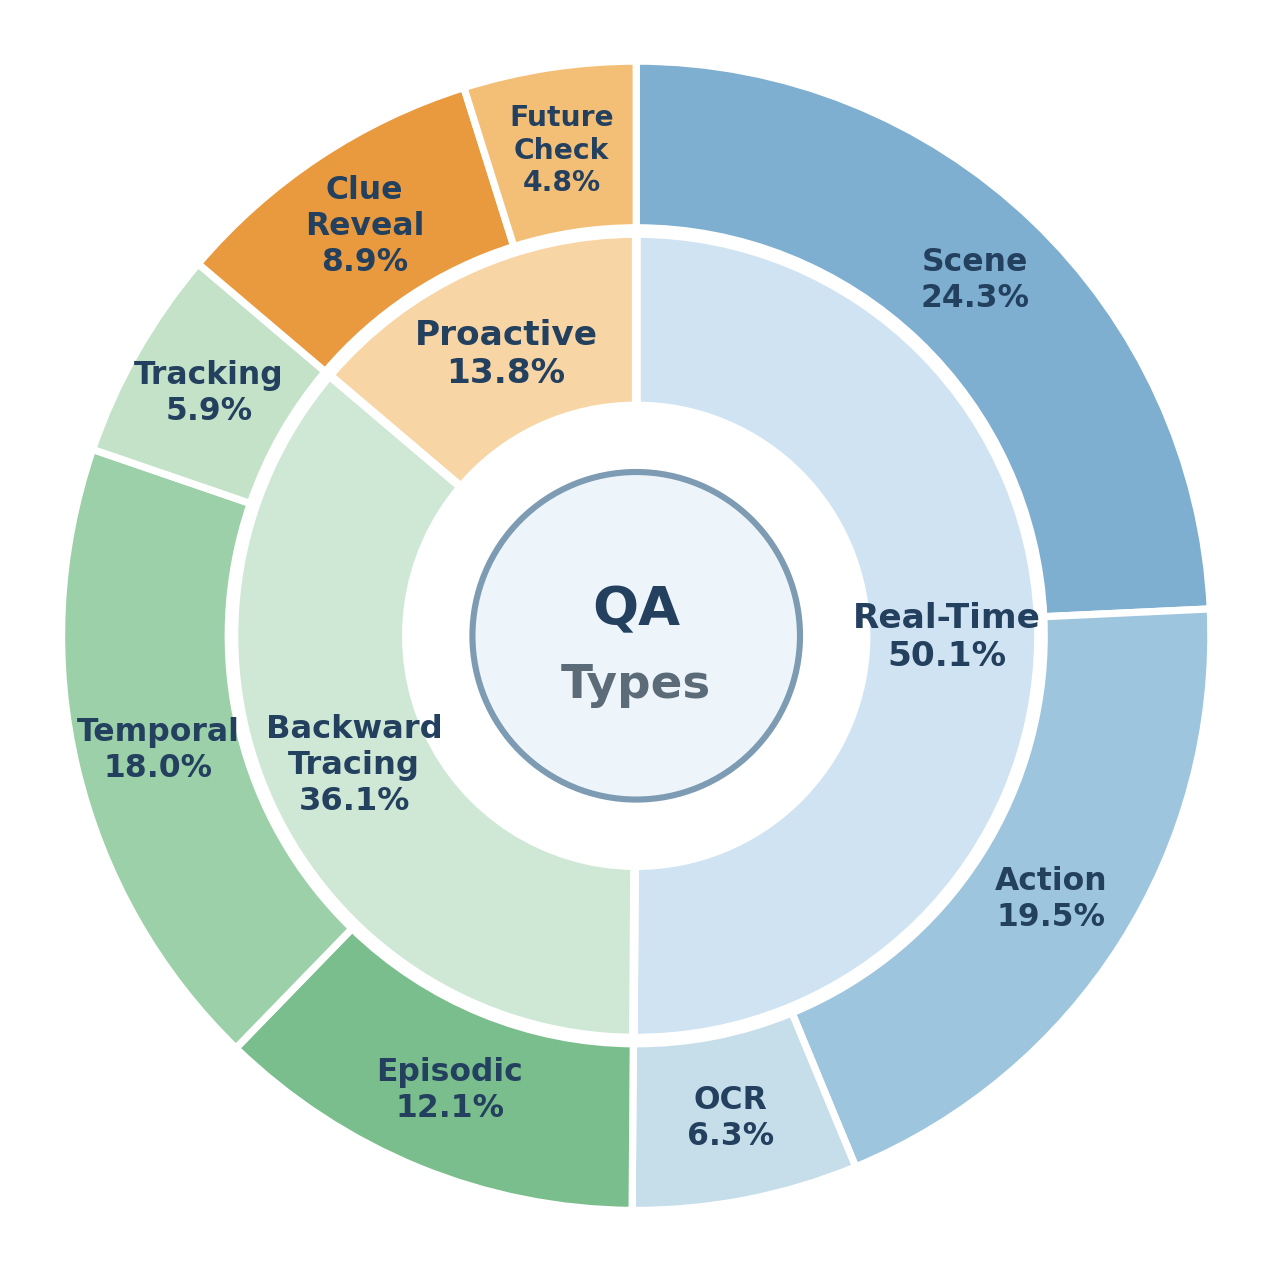
\includegraphics[width=0.92\columnwidth]{figures/figure_qa_distribution.png}
  \caption{Distribution of constructed questions by streaming mode and task focus.}
  \label{fig:data_question_distribution}
\end{figure}
